\chapter{Introduction}

\label{chap:introduction}
\section{Eye Tracking}
Eye-tracking is utilised to monitor eye movement. It is employed in a wide variety of fields such as marketing research, psychology, virtual reality and sports. In sport research eye-tracking offers important insights about the hand-eye coordination or visual search techniques. These differ greatly between professional athletes and beginners so the analysis can improve the efficiency of training. 

An eye-tracking device for sports needs a high accuracy and temporal resolution to draw accurate conclusions. As the device should interfere as little as possible with the activity of an athlete, it should also be portable.

\section{Current State}
In collaboration with the sport research institute at the University of Bern, the microLab research group has developed an eye-tracking system for sports. This system utilizes two cameras per eye to capture infrared images at a high speed of 120 frames per second. The information from the cameras should be used to determine the gaze direction of the athlete. An important part of that is the detection of the pupil, which is not implemented satisfactory yet.

\section{Overview of the Eye-tracking System}
The Gazelle eye-tracking system consists of two main parts. The first is the GazelleGlasses where the cameras are mounted and the data is sent down to the second main part which is GazelleCompute. As the name suggests this component is responsible for the processing of the data.

\subsubsection{GazelleGlasses}
For the capture of an eye two cameras are placed below the eye and besides the nose. This positioning was chosen to not obstruct the view of the athlete and offer a good perspective on the eye. A front facing camera is placed between the eyes and provides a view that is close to the view of the athlete.

The data that is generated by the cameras needs to be transferred to GazelleCompute. This is done by serializing the data and sending it over an Ethernet cable to the main compute unit.
\subsubsection{GazelleCompute}
The main processing is done on a small portable unit. The units main components are a Zynq FPGA and a Tegra 3. Initially the idea was to do the image processing on the Tegra 3 as it is a powerfull mobile System on Chip.

Problems with the data transfer from the FPGA to the Tegra 3 scrambled that idea. The image processing is now required to run on the dual core arm CPU that is on the Zynq FPGA.
\section{Pupil Detection}

\section{Organising Documents}
\label{sec:einleitung_aufbau}

This document is structured according to the documentation of a project work or a thesis\index{thesis}. In Chapter \ref{chap:instructions}, the packages used are briefly explained, and instructions are given, how the bibliography and the glossary are to be used. Chapter \ref{chap:typeareatest} presents a sample chapter to audit the type area.

In figure \ref{fig:file_structure} the file structure is shown for this template.

\begin{figure}[H]
	\centering
		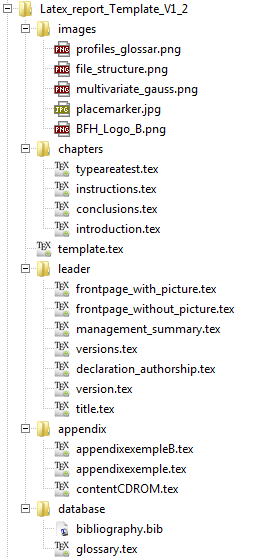
\includegraphics[scale=0.85]{images/file_structure.png}
	\caption{File structure}
	\label{fig:file_structure}
\end{figure}

\section{Contact}
\label{sec:introduction_contact}

The manufacturers of this template welcome any suggestions for improvement. Chapter \ref{sec:introduction_suggestions} shows possible suggestions for improvement\index{suggestions}.

\begin{table}[H]
	\centering
		\begin{tabular}{lll} \toprule
			\textbf{First Name Last Name} & \textbf{E-mail} & \textbf{Function} \\ \midrule
			Alfred Kaufmann & alfred.kaufmann@bfh.ch & Employer, Project Management, \\
			& & Supplements, Improvements \\ \midrule
			Fritz Dellsperger & Retired & Tips on the structure and layout \\ \midrule
			David Burri & Contracted out & First compilation of the Template \\ \bottomrule
		\end{tabular}
	\caption{Contact Persons}
	\label{tab:Contact Persons}
\end{table}


\section{Suggestions for Improvement}
\label{sec:introduction_suggestions}

\begin{itemize}
	\item Create a BFH Style Files
	\item Template for the Compilation of presentations with \LaTeX{}
\end{itemize}


